{\noindent 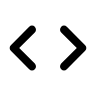
\includegraphics[scale=\categoryIconScale]{round_code_black_48dp} \hspace{0.25pc} \large Open Source and Presentations}\hspace{1pc}{\noindent\rule{29pc}{0.4pt}}

\begin{itemize}
	\setlength{\itemsep}{0.0pc}
	\item[] \textbf{TOXIC} - Task Execution Engine\hspace{22pc}{\secondaryColor
	\href{https://github.com/stackct/toxic}{github.com/stackct/toxic}}
	
	\item[] \textbf{rotor.ai} - Open Source Self-Driving Project\hspace{24.75pc}{\secondaryColor \href{https://rotor.ai}{rotor.ai}}
	
	\item[] {\it Practical TDD with Dart\texttrademark \& Flutter\texttrademark}\hspace{15.5pc}{\secondaryColor \href{https://rotor.ai/blog/2019/4/28/tdd-flutter-sdk}{rotor.ai/blog/2019/4/28/tdd-flutter-sdk}}
	
	%\item[] \textbf{Rsolver} - Rubik's Cube AI \hspace{22.5pc} {\secondaryColor \href{https://www.github.com/stuartsoft/RSolver}{github.com/stuartsoft/RSolver}}
	
	\item[] \textbf{Carbon Android} - Android starter project\hspace{13.15pc}
	{\secondaryColor{\href{https://github.com/atomicrobot/carbon-android}{github.com/atomicrobot/carbon-android}}}	
\end{itemize}
